\documentclass[aspectratio=169,11pt]{beamer}
\usetheme{metropolis}
\usepackage{listings}
\usepackage{tikz}
\usepackage{amsmath,amssymb,amsthm}
\usepackage{xcolor}
\usepackage{stmaryrd}
\usepackage{mathtools}

\usetikzlibrary{arrows.meta, positioning, calc, decorations.pathreplacing, shapes.geometric, cd}

% Colors
\definecolor{siteA}{HTML}{4C72B0}
\definecolor{siteB}{HTML}{DD8452}
\definecolor{siteC}{HTML}{55A868}
\definecolor{conflict}{HTML}{C44E52}
\definecolor{ok}{HTML}{55A868}
\definecolor{codebg}{HTML}{F5F5F5}

\lstset{
  basicstyle=\ttfamily\scriptsize,
  backgroundcolor=\color{codebg},
  frame=single,
  framerule=0pt,
  columns=fullflexible,
  keepspaces=true,
  escapeinside={(*}{*)},
  keywordstyle=\color{siteA}\bfseries,
  stringstyle=\color{siteB},
  commentstyle=\color{gray}\itshape,
  language=Python,
  morekeywords={deppy,requires,guarantee},
  showstringspaces=false,
}

\newcommand{\Sem}{\mathcal{F}}
\newcommand{\Cov}{\mathfrak{C}}
\newcommand{\Cat}{\mathbf{S}}
\newcommand{\Poset}{\mathbf{Poset}}
\newcommand{\Set}{\mathbf{Set}}
\newcommand{\op}{\mathrm{op}}

\title{\textbf{DepPy}: Sheaf-Descent Semantic Typing\\for Python Programs}
\subtitle{Local type facts, gluing axioms, and cohomological bug detection}
\author{Halley Young}
\date{}

\begin{document}

% ══════════════════════════════════════════════════════════════════════════════
% TITLE
% ══════════════════════════════════════════════════════════════════════════════
\begin{frame}
\titlepage
\end{frame}

% ══════════════════════════════════════════════════════════════════════════════
% SLIDE 1: Motivation — The Local-to-Global Problem
% ══════════════════════════════════════════════════════════════════════════════
\begin{frame}{The Local-to-Global Problem in Program Analysis}

Every program analysis asks a \emph{local-to-global} question:

\vspace{0.3em}
\begin{center}
\begin{tabular}{@{}lll@{}}
\textbf{Technique} & \textbf{Local data} & \textbf{Global assembly} \\
\hline
Type checking    & Per-expression judgments $\Gamma \vdash e : \tau$ & Compose via typing rules \\
Abstract interp. & Transfer functions per block & Fixed-point over lattice \\
Hoare logic      & $\{P\}\; c\; \{Q\}$ per statement & Sequential composition \\
Model checking   & Per-state transitions & Reachability / B\"uchi \\
Refinement types & Per-binding refinements & Subtyping + SMT \\
\end{tabular}
\end{center}

\vspace{0.4em}
\textbf{Observation:} each technique invents its own gluing mechanism.

\vspace{0.3em}
\textbf{Sheaf theory} is the mathematical theory of \emph{exactly this problem}:
given compatible local data on overlapping open sets, when does a
unique global object exist?

\vspace{0.3em}
{\small \textbf{This talk:} we instantiate sheaves over a site category of program points,
and show that type consistency, behavioral equivalence, spec verification, and
bug detection all reduce to the \emph{same} sheaf-theoretic operation — checking
whether local sections glue.}

\end{frame}

% ══════════════════════════════════════════════════════════════════════════════
% SLIDE 2: Sites, Presheaves, Sections
% ══════════════════════════════════════════════════════════════════════════════
\begin{frame}[fragile]{Sites, Presheaves, and Sections}

\begin{columns}[T]
\column{0.52\textwidth}

\textbf{Definition.} A \emph{site category} $\Cat$ has:
\begin{itemize}
  \item \textbf{Objects} = program observation points (\emph{sites})
  \item \textbf{Morphisms} = data-flow / control-flow edges
\end{itemize}

A \emph{presheaf} is a contravariant functor
$\Sem : \Cat^{\op} \to \Poset$:
\begin{itemize}
  \item $\Sem(U)$ = set of type facts observable at site $U$
  \item For $f : V \to U$, the \emph{restriction} $\Sem(f) : \Sem(U) \to \Sem(V)$ propagates facts along edges
\end{itemize}

A \emph{section} $\sigma \in \Sem(U)$ is a concrete type fact at site $U$.

\column{0.44\textwidth}

\begin{lstlisting}
def average(xs: list[int]) -> float:
    total = sum(xs)       # site U1
    n = len(xs)           # site U2
    return total / n      # site U3
\end{lstlisting}

\vspace{0.3em}
{\small
\begin{tabular}{@{}ll@{}}
\textbf{Site} & \textbf{Section $\sigma \in \Sem(U)$} \\
\hline
$U_1$ & \texttt{xs : list[int]} \\
$U_2$ & \texttt{n : int} \\
$U_3$ & \texttt{/ } needs \texttt{n $\neq$ 0} \\
\end{tabular}
}

\vspace{0.3em}
{\small DepPy defines \textbf{14 site families} (\texttt{SiteKind}):
argument boundary, return boundary, SSA value,
branch guard, call result, tensor shape/order/indexing,
heap protocol, proof, trace, error, loop header invariant,
module summary.}

\vspace{0.3em}
{\small Each section is a \texttt{LocalSection}: carrier type, refinement predicates,
trust level, provenance, witnesses.}

\end{columns}

\end{frame}

% ══════════════════════════════════════════════════════════════════════════════
% SLIDE 3: Covers and the Sheaf Condition
% ══════════════════════════════════════════════════════════════════════════════
\begin{frame}{Covers and the Sheaf Condition}

\textbf{Definition.} A \emph{cover} of site $U$ is a family
$\{U_i \to U\}_{i \in I}$ with overlap data
$U_i \cap U_j$ for each pair.

\vspace{0.3em}
\textbf{The sheaf condition} (equalizer formulation):
given sections $\sigma_i \in \Sem(U_i)$ such that
$\sigma_i|_{U_i \cap U_j} = \sigma_j|_{U_i \cap U_j}$
for all $i, j$, there exists a \emph{unique} global section
$\sigma \in \Sem(U)$ with $\sigma|_{U_i} = \sigma_i$.

\vspace{0.3em}
\begin{center}
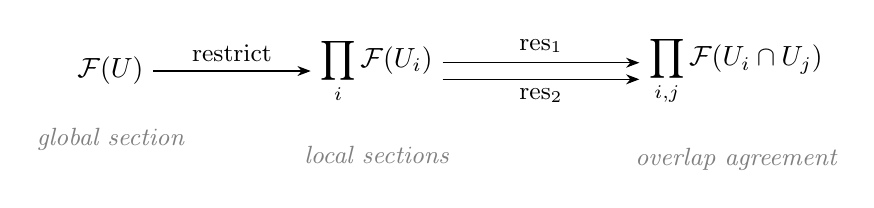
\begin{tikzpicture}[>=Stealth, node distance=1.8cm]
  \node (FU) {$\Sem(U)$};
  \node[right=2cm of FU] (prod) {$\displaystyle\prod_i \Sem(U_i)$};
  \node[right=2.5cm of prod] (coprod) {$\displaystyle\prod_{i,j} \Sem(U_i \cap U_j)$};
  
  \draw[->] (FU) -- node[above, font=\small] {restrict} (prod);
  \draw[->, transform canvas={yshift=3pt}] (prod) -- node[above, font=\small] {$\mathrm{res}_1$} (coprod);
  \draw[->, transform canvas={yshift=-3pt}] (prod) -- node[below, font=\small] {$\mathrm{res}_2$} (coprod);
  
  \node[below=0.3cm of FU, font=\small\itshape, text=gray] {global section};
  \node[below=0.3cm of prod, font=\small\itshape, text=gray] {local sections};
  \node[below=0.3cm of coprod, font=\small\itshape, text=gray] {overlap agreement};
\end{tikzpicture}
\end{center}

\vspace{0.2em}
\textbf{PL reading:} the global section \emph{is} a consistent whole-program typing.
The equalizer diagram says: local type judgments compose into a global judgment
\emph{iff} they agree on shared variables.

\vspace{0.3em}
{\small \textbf{Implementation:} \texttt{SheafConditionChecker} checks
\texttt{check\_agreement} (pairwise compatibility on overlaps),
\texttt{attempt\_gluing} (construct \texttt{GlobalSection}),
and \texttt{verify\_uniqueness} (restriction recovers each local).}

\end{frame}

% ══════════════════════════════════════════════════════════════════════════════
% SLIDE 4: Grothendieck Topology
% ══════════════════════════════════════════════════════════════════════════════
\begin{frame}{Grothendieck Topology on Program Sites}

A \emph{Grothendieck topology} $J$ on $\Cat$ assigns to each site $U$ a
collection of covering families $\Cov(U)$ satisfying three axioms:

\vspace{0.3em}
\begin{enumerate}
  \item \textbf{Identity:} $\{U \xrightarrow{\mathrm{id}} U\} \in \Cov(U)$ \hfill
        {\small (trivial cover)}
  \item \textbf{Stability:} if $\{U_i \to U\} \in \Cov(U)$ and $V \to U$,
        then $\{U_i \times_U V \to V\} \in \Cov(V)$ \hfill
        {\small (pullback)}
  \item \textbf{Transitivity:} if $\{U_i \to U\} \in \Cov(U)$ and
        $\{V_{ij} \to U_i\} \in \Cov(U_i)$ for each $i$, then
        $\{V_{ij} \to U\} \in \Cov(U)$ \hfill
        {\small (refinement)}
\end{enumerate}

\vspace{0.3em}
\textbf{PL reading:}

\vspace{0.2em}
{\small
\begin{tabular}{@{}lll@{}}
\textbf{Axiom} & \textbf{PL interpretation} & \textbf{Analogy} \\
\hline
Identity     & A function is covered by itself          & Trivial self-analysis \\
Stability    & Analysis is stable under specialization  & Restrict to a call-site \\
Transitivity & Inlining preserves coverage              & Interprocedural analysis \\
\end{tabular}
}

\vspace{0.4em}
{\small \textbf{Implementation:} \texttt{ConcreteTopolgy} stores covers indexed by site;
\texttt{is\_cover} checks \texttt{\_check\_identity}, \texttt{\_check\_stability},
\texttt{\_check\_transitivity} in sequence.
The topology ensures that DepPy's analysis is stable under function inlining,
specialization, and modular composition.}

\end{frame}

% ══════════════════════════════════════════════════════════════════════════════
% SLIDE 5: Obstructions and Čech Cohomology
% ══════════════════════════════════════════════════════════════════════════════
\begin{frame}{Obstructions and \v{C}ech Cohomology}

When the sheaf condition \emph{fails}, the failure is classified by
\textbf{\v{C}ech cohomology}:

\vspace{0.3em}
{\small
\begin{tabular}{@{}lll@{}}
\textbf{Degree} & \textbf{Mathematical meaning} & \textbf{PL meaning} \\
\hline
$H^0(\mathcal{U}, \Sem)$ & Global sections & Consistent whole-program typing \\
$H^1(\mathcal{U}, \Sem)$ & Gluing obstructions & \textbf{Type errors / bugs} \\
$H^2(\mathcal{U}, \Sem)$ & Higher obstructions & (Higher-order inconsistencies) \\
\end{tabular}
}

\vspace{0.3em}
An \textbf{obstruction} $[\alpha] \in H^1(\mathcal{U}, \Sem)$ is a
\v{C}ech 1-cocycle: a pair of overlapping sites $(U_i, U_j)$
where sections cannot be reconciled.

\vspace{0.3em}
\textbf{Key insight:} the obstruction \emph{localizes} the bug.
It names the exact pair of sites where local type facts conflict — not
just ``the program has a type error.''

\vspace{0.4em}
{\small
\textbf{Implementation:}
\texttt{ObstructionData} stores a \texttt{CohomologyClass} (degree, representative cochain, triviality flag)
and \texttt{conflicting\_overlaps: List[Tuple[SiteId, SiteId]]}.
The representative cochain gives a concrete witness of the inconsistency.
}

\vspace{0.3em}
{\small
\textbf{Seven obstruction families} (\texttt{ObstructionFamily}):
\textsc{RefinementGap}, \textsc{CarrierMismatch}, \textsc{TaintLeakage},
\textsc{ProtocolViolation}, \textsc{ResourceLifetime},
\textsc{ConfigurationWeakness}, \textsc{ExceptionEscapement}.
Each maps a class of bugs to a specific presheaf failure mode.
}

\end{frame}

% ══════════════════════════════════════════════════════════════════════════════
% SLIDE 6: Behavioral Equivalence — Theory
% ══════════════════════════════════════════════════════════════════════════════
\begin{frame}{Behavioral Equivalence via Sheaf Morphisms}

\textbf{Setup.} Given programs $f, g$, build presheaves
$\Sem_f, \Sem_g : \Cat^{\op} \to \Poset$ over a common site
refinement. Behavioral equivalence becomes:

\vspace{0.2em}
\begin{center}
\emph{Does a natural isomorphism $\eta : \Sem_f \xrightarrow{\sim} \Sem_g$ exist?}
\end{center}

\vspace{0.2em}
\textbf{6-phase pipeline} (from \texttt{GlobalEquivalenceChecker}):

{\small
\begin{enumerate}
  \item \textbf{Local checking:} for each site $U_i$ in the common refinement, check
        $\Sem_f(U_i) \cong \Sem_g(U_i)$ via \texttt{LocalEquivalenceChecker}
  \item \textbf{Naturality:} verify local isomorphisms form a natural transformation —
        all naturality squares commute (\texttt{SheafMorphismBuilder})
  \item \textbf{Descent ($H^1$):} compute $H^1(\mathcal{U},\, \mathrm{Iso}(\Sem_f, \Sem_g))$;
        descent holds iff $H^1 = 0$ (\texttt{EquivalenceDescentChecker})
  \item \textbf{Gluing:} construct global equivalence via fiber product
        $\Sem_f \times_{\Cat} \Sem_g$ (\texttt{FiberProductBuilder})
  \item \textbf{Uniqueness:} verify the glued section is unique (sheaf condition)
  \item \textbf{Stalk verification} (optional): cross-check that
        $\eta_p$ is a bijection at all stalks $p$
\end{enumerate}
}

\vspace{0.3em}
\textbf{Comparison with standard PL:}

{\small
\begin{tabular}{@{}ll@{}}
Bisimulation relation $R$ (global, up-front) & $\longleftrightarrow$ Presheaf morphism $\eta$ (local, composable) \\
Relational Hoare: aligned loop invariants & $\longleftrightarrow$ Sections at loop-header sites \\
Contextual equivalence: $\forall C.\; C[f] \simeq C[g]$ & $\longleftrightarrow$ Stalk iso at all points (Phase 6) \\
\end{tabular}
}

\end{frame}

% ══════════════════════════════════════════════════════════════════════════════
% SLIDE 7: Behavioral Equivalence — Code
% ══════════════════════════════════════════════════════════════════════════════
\begin{frame}[fragile]{Behavioral Equivalence: Implementation}

\begin{columns}[T]
\column{0.46\textwidth}

\textbf{Problem.} Given $f, g$ with different implementations, decide
$\forall x.\; f(x) = g(x)$ and localize any divergence.

\vspace{0.3em}
\textbf{Standard approach} — testing or relational Hoare:

\begin{lstlisting}
# Property-based: incomplete
for xs in random_inputs():
    assert sort_v1(xs) == sort_v2(xs)

# Relational Hoare: need global
# alignment + loop invariants
\end{lstlisting}

{\small Bisimulation requires constructing $R$ globally.
Logical relations give compositionality but are
typically manual and target-language-specific.}

\column{0.50\textwidth}

\textbf{DepPy} — local checks, sheaf gluing:

\begin{lstlisting}
from deppy.equivalence.pipeline import (
    EquivalencePipeline,
    EquivalencePipelineConfig,
)

pipe = EquivalencePipeline(
    EquivalencePipelineConfig(
        function_name="sort_values"))

result = pipe.run("sort_v1.py",
                  "sort_v2.py")

print(result.is_equivalent)
print(result.verdict)
# If INEQUIVALENT:
#   result.obstructions[0].sites
#   -> exact divergence site
#   result.descent_result
#   -> H^1 witness
\end{lstlisting}

\end{columns}

\vspace{0.2em}
{\small The pipeline returns \texttt{GlobalEquivalenceResult} with
\texttt{local\_judgments}, \texttt{sheaf\_morphism} (naturality data),
\texttt{descent\_result} ($H^1$ computation), and \texttt{stalk\_result}.}

\end{frame}

% ══════════════════════════════════════════════════════════════════════════════
% SLIDE 8: Spec Checking — Čech Descent Theory
% ══════════════════════════════════════════════════════════════════════════════
\begin{frame}{Spec Checking via \v{C}ech Descent}

\textbf{Setup.} Given implementation $I$ with $k$ paths $\{P_i\}$ and
spec $S = C_1 \wedge \cdots \wedge C_m$ (conjunction of predicates),
define the \emph{spec presheaf} $\Sem_S$:
\[
  \Sem_S(U) \;=\; \{(x, y) \mid x \in U,\; S(x, y)\}
\]

\textbf{Verification question:} does the section
$\sigma : x \mapsto (x, I(x))$ lie in $\Gamma(X, \Sem_S)$?

\vspace{0.3em}
\textbf{Product cover.}
$\mathcal{U} = \{(P_i, C_j)\}_{i \le k,\, j \le m}$ with
$|\mathcal{U}| = k \times m$ sites. Each site generates a VC:
\[
  \mathrm{VC}_{i,j} \;=\; \forall x \in P_i.\; C_j(x, \sigma_i(x))
\]

\textbf{Standard VCGen} solves all $k \times m$ VCs independently.
DepPy does three optimizations via the \textbf{\v{C}ech nerve}
$N(\mathcal{U})$:

{\small
\begin{enumerate}
  \item \textbf{$H^1$ elimination:} compute $\dim H^1 = |E| - |V| + |\pi_0|$
        of the nerve; each independent cycle identifies a \emph{redundant} VC
        (one VC per cycle can be dropped)
  \item \textbf{$H^0$ proof transfer:} within each connected component,
        proving \emph{any} site with conjunct $C_j$ proves \emph{all} sites
        with $C_j$ (sheaf gluing propagation)
  \item \textbf{Mayer--Vietoris decomposition:} for each conjunct, identify
        independent path groups with trivial $H^1$ contribution
\end{enumerate}
}

\vspace{0.2em}
{\small The net effect: VC count drops from $O(k \cdot m)$ to
$O(|\text{overlaps}|)$ in practice.}

\end{frame}

% ══════════════════════════════════════════════════════════════════════════════
% SLIDE 9: Spec Checking — Layered Proof Strategy
% ══════════════════════════════════════════════════════════════════════════════
\begin{frame}{Spec Checking: Layered Proof Strategy}

The \texttt{SheafSpecVerifier} descends through the \v{C}ech-to-derived
functor spectral sequence in five layers:

\vspace{0.3em}
{\small
\begin{tabular}{@{}clp{7.5cm}@{}}
\textbf{Layer} & \textbf{Name} & \textbf{Description} \\
\hline
0 & $H^1$ \v{C}ech elimination & Remove redundant VCs via nerve cycle detection \\
1 & Structural proof (stalk) & Prove VCs by matching implementation structure to spec structure at stalks \\
2 & Section existence via Z3 & Discharge remaining VCs with SMT queries \\
3 & $H^0$ sheaf transfer & Propagate successful proofs to equivalent sites via gluing \\
4 & Spec-only Z3 & Final tautology / refutation check on residual obligations \\
\end{tabular}
}

\vspace{0.4em}
\textbf{Pipeline phases} (from \texttt{SheafSpecVerifier.verify}):

{\small
\begin{enumerate}
  \item Compile spec to formal predicate AST
  \item Decompose spec presheaf: $S = C_1 \wedge \cdots \wedge C_k$
        (\texttt{decompose\_spec} $\to$ \texttt{SpecDecomposition} with conjuncts + overlap graph)
  \item Analyze implementation cover $\{P_i\}$ (path enumeration)
  \item Build product cover $P \times C$ and \v{C}ech nerve (\texttt{build\_sheaf\_cover} $\to$ \texttt{SheafCover} with \texttt{CechComplex})
  \item Symbolically execute implementation paths
  \item Sheaf descent: apply layers 0--4 in sequence
\end{enumerate}
}

\vspace{0.2em}
{\small \textbf{Key data structure:} \texttt{CechComplex} stores
\texttt{n\_vertices}, \texttt{edges}, \texttt{n\_components}, \texttt{h1\_dimension},
\texttt{independent\_cycles} — the full simplicial structure of the nerve.}

\end{frame}

% ══════════════════════════════════════════════════════════════════════════════
% SLIDE 10: Spec Checking — Code + 100 Algorithms
% ══════════════════════════════════════════════════════════════════════════════
\begin{frame}[fragile]{Spec Checking: 100-Algorithm Evaluation}

\begin{columns}[T]
\column{0.46\textwidth}

\textbf{Problem.} Given $I$ and spec $S : \mathit{In} \times \mathit{Out} \to \mathbb{B}$, decide
$\forall x.\; S(x, I(x))$.
Reject if a concrete counterexample or $H^1$ obstruction is found.

\vspace{0.3em}
\textbf{Standard:} Hypothesis / QuickCheck:

\begin{lstlisting}
from hypothesis import given, strategies
@given(strategies.lists(
        strategies.integers()))
def test_sort(arr):
    result = solve(arr)
    assert result == sorted(arr)
    assert len(result) == len(arr)
\end{lstlisting}

{\small Incomplete — misses rare inputs.
Hoare VCGen gives a proof but has
$O(|\text{paths}|)$ VCs per conjunct.}

\column{0.50\textwidth}

\textbf{DepPy} — sheaf-descent verification:

\begin{lstlisting}
from deppy.render.predicate_refine import (
    SheafSpecVerifier)

def sort_spec(arr, result):
    return (result == sorted(arr)
            and len(result) == len(arr))

v = SheafSpecVerifier(z3_timeout_ms=3000)

r = v.verify(correct_source, sort_spec)
print(r.correct)   # True

r = v.verify(buggy_source, sort_spec,
    reference_source=correct_source)
print(r.refuted)   # True
# r.cover -> SheafCover with CechComplex
# r.cover.cech.h1_dimension -> int
# r.eliminated_vcs -> count
\end{lstlisting}

\end{columns}

\vspace{0.3em}
{\small \textbf{Evaluation:} 100 algorithms (Tarjan SCC, Dinic flow, KD-tree, Fibonacci heap, Z-algorithm, \ldots).
Each has a \texttt{CORRECT} and subtly \texttt{BUGGY} variant sharing one \texttt{SPEC} predicate.
Same \texttt{SheafSpecVerifier} pipeline, no per-algorithm tuning.}

\end{frame}

% ══════════════════════════════════════════════════════════════════════════════
% SLIDE 11: Bug Finding — Unified Obstruction Framework
% ══════════════════════════════════════════════════════════════════════════════
\begin{frame}{Bug Finding: Obstructions as a Unifying Framework}

\textbf{Claim:} diverse bug classes are \emph{all} gluing obstructions — they differ
only in \emph{which presheaf} fails to glue.

\vspace{0.3em}
{\small
\begin{tabular}{@{}llll@{}}
\textbf{Obstruction family} & \textbf{Presheaf} & \textbf{Bug classes} & \textbf{Standard tool} \\
\hline
\textsc{RefinementGap} & Refinement predicate $\{x \mid \varphi(x)\}$ &
  \texttt{DIV\_ZERO}, \texttt{NULL\_PTR}, \texttt{INDEX\_OOB}, & Nullable / bounds \\
  & & \texttt{ASSERT\_FAIL}, \texttt{OVERFLOW}, \texttt{BOUNDS} & analysis, lint \\[2pt]
\textsc{CarrierMismatch} & Carrier type $\tau$ at site &
  \texttt{TYPE\_ERROR}, \texttt{TYPE\_CONFUSION} & Type checker \\[2pt]
\textsc{TaintLeakage} & Secrecy label $\ell \in \mathcal{L}$ &
  \texttt{INFO\_LEAK} & Taint analysis \\[2pt]
\textsc{ProtocolViolation} & State machine presheaf &
  \texttt{DEADLOCK}, \texttt{DATA\_RACE} & Lock-order / race \\
  & & \texttt{ITERATOR\_PROTOCOL} & detector \\[2pt]
\textsc{ResourceLifetime} & Resource lifecycle $\mathrm{open} \to \mathrm{closed}$ &
  \texttt{MEMORY\_LEAK}, \texttt{USE\_AFTER\_FREE}, & Leak sanitizer / \\
  & & \texttt{DOUBLE\_FREE} & lifetime analysis \\[2pt]
\textsc{ConfigWeakness} & Config-space presheaf &
  \texttt{WEAK\_CRYPTO} & Security audit \\[2pt]
\textsc{ExceptionEscape} & Exception presheaf &
  \texttt{RUNTIME\_ERROR}, \texttt{UNBOUND\_VAR}, & Exception analysis, \\
  & & \texttt{KEY\_ERROR}, \texttt{NON\_TERMINATION} & termination checker \\
\end{tabular}
}

\vspace{0.3em}
{\small \textbf{The pipeline is invariant:} build cover $\to$ assign sections of the
relevant presheaf $\to$ check gluing $\to$ report obstruction class $[\alpha] \in H^1$.
The bug class selects the presheaf; the machinery is reused.}

\end{frame}

% ══════════════════════════════════════════════════════════════════════════════
% SLIDE 12: Bug Finding — Code + 20 Bug Classes
% ══════════════════════════════════════════════════════════════════════════════
\begin{frame}[fragile]{Bug Finding: 20 Bug Classes, One Pipeline}

\begin{columns}[T]
\column{0.46\textwidth}

\textbf{Problem.} Detect bugs across 20 categories without
a separate analysis per category.

\vspace{0.3em}
\textbf{Standard:} compose $n$ tools, each with its own IR:

\begin{lstlisting}
# mypy  -> types
# pylint -> style + some bugs
# bandit -> security
# ASAN   -> memory
# TSAN   -> concurrency
# Valgrind -> leaks
# ...10+ tools, each with own
#    abstraction & false-positive
#    profile
\end{lstlisting}

{\small No shared formalism.
Adding a new bug class = building a new tool
from scratch.}

\column{0.50\textwidth}

\textbf{DepPy} — one obstruction framework:

\begin{lstlisting}
from deppy.render.bug_detect import (
    detect_bugs, format_bug_report)

source = """
def swap_first_last(lst):
    tmp = lst[0]
    lst[0] = lst[len(lst)-1]
    lst[len(lst)-1] = tmp
    return lst
"""

report = detect_bugs(source)
print(report.bugs_found)  # 1
for ob in report.obstructions:
    print(ob.bug_type,   # INDEX_OOB
          ob.line,        # 3
          ob.confidence,  # 0.85
          ob.family)      # REFINEMENT_GAP
# format_bug_report(report) ->
#   human-readable with family,
#   CWE, conflicting sites
\end{lstlisting}

\end{columns}

\vspace{0.2em}
{\small \textbf{Evaluation:} 20 bug classes, each with buggy/safe pairs from
\texttt{synthetic\_bug\_suite} (40 programs).
Adding a new bug class = defining a new presheaf + registering in \texttt{BUG\_SPECS}.
The \texttt{detect\_bugs} entry point dispatches by \texttt{ObstructionFamily}:
\textsc{TaintLeakage} $\to$ taint-specific discharge;
all others $\to$ generic Z3 obstruction discharge.}

\end{frame}

% ══════════════════════════════════════════════════════════════════════════════
% SLIDE 13: Related Work and Discussion
% ══════════════════════════════════════════════════════════════════════════════
\begin{frame}{Related Work and Discussion}

\begin{columns}[T]
\column{0.48\textwidth}

\textbf{Connections to existing PL work:}

\vspace{0.3em}
{\small
\begin{tabular}{@{}lp{4cm}@{}}
\textbf{Area} & \textbf{Relationship} \\
\hline
Abstract interp. & Local sections $\approx$ abstract values;
  gluing $\approx$ join/widen at merge points \\[3pt]
Refinement types & Sections carry refinements $\{x \mid \varphi\}$;
  overlap $\approx$ subtyping query to SMT \\[3pt]
Separation logic & Frame rule $\approx$ restriction along morphisms;
  $*$ $\approx$ disjoint union of sites \\[3pt]
Liquid Haskell & Spec predicates $\approx$ liquid types;
  \v{C}ech elimination $\approx$ qualifier minimization \\[3pt]
Logical relations & Stalk verification $\approx$ fundamental theorem of logical relations \\
\end{tabular}
}

\column{0.48\textwidth}

\textbf{What does sheaf theory buy?}

\vspace{0.3em}
\begin{enumerate}
  \item \textbf{Unification:} equivalence, spec checking, and bug finding share one pipeline
  \item \textbf{Localization:} obstructions name the exact conflicting site pair, not just ``type error on line $n$''
  \item \textbf{VC reduction:} \v{C}ech $H^1$ elimination + $H^0$ transfer reduce verification obligations vs.\ path-based VCGen
  \item \textbf{Extensibility:} new bug class = new presheaf + registration, not a new tool
  \item \textbf{Formal backbone:} Grothendieck axioms guarantee that analysis composes under inlining, specialization, and modular linking
\end{enumerate}

\end{columns}

\vspace{0.4em}
{\small \textbf{Evaluation summary:} 100-algorithm spec suite, 20-bug-class detection suite (40 programs),
behavioral equivalence on implementation variants.
All three tasks use the same core: cover $\to$ sections $\to$ gluing $\to$ obstruction.}

\end{frame}

\end{document}
